JWT steht für "JSON Web Token" und repräsentiert einen offenen Standard (RFC 7519). Er ist zur Authentifizierung und Autorisierung gedacht, dieser Token kann sowohl vom Server als auch vom Client ausgelesen werden. Er kann verwendet werden um Daten sicher zwischen verschiedenen Anwendungen zu übermitteln. Durch die Signatur des JWT kann immer sichergestellt werden, dass nichts vom Inhalt manipuliert wurde.


\subsection{Wie ist ein JWT aufgebaut?}
Ein JWT ist grundlegend in drei Bereiche gegliedert:

\begin{itemize}
\item \textbf{Header}
\item \textbf{Payload}
\item \textbf{Signatur}
\end{itemize}

\begin{figure}[h!]
    \centering
    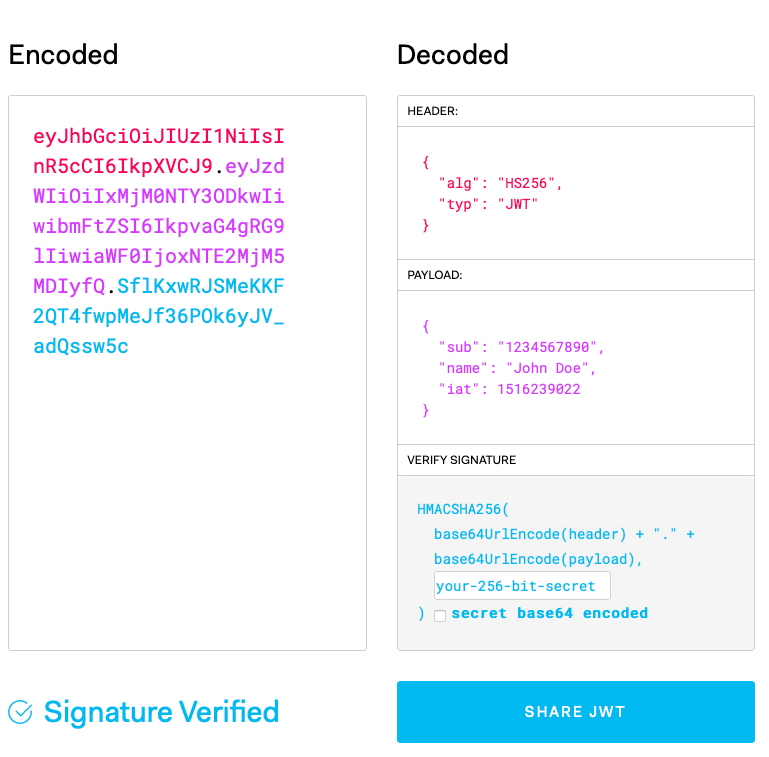
\includegraphics[width=0.6\textwidth]{pics/jwt.png}
    \caption{JSON Web Token}
    \label{fig:enter-label}
\end{figure}

\subsection{Session vs. JSON Web Token}


Der Header wird auch als JOSE (JSON Object Signing and Encryption) bezeichnet. In diesem sind ausschließlich Informationen über die Signierung und Verschlüsselung des JWT enthalten.

Typischerweise enthält die Struktur eines JWT-Headers eine Information über den Algorithmus, welcher zur Erstellung der Signatur verwendet wurde, sowie eine Definition, dass es sich um ein Json Web Token handelt. Dabei ist zu beachten, dass die Angabe des Typs optional ist, jedoch häufig auf "JWT" festgelegt wird. Dies ist besonders relevant für Anwendungen, die auch andere Typen, wie beispielsweise einen Access Token, akzeptieren, welcher jedoch in einer ähnlichen Datenstruktur vorliegt, um die verschiedenen Typen leicht voneinander unterscheiden zu können.

\begin{lstlisting}
    {
  "alg": "HS256",
  "typ": "JWT"
}
\end{lstlisting}

Der zweite Part des JSON Web Token ist die Payload. Diese beinhaltet drei verschiedene Arten von Claims. 
Registrierte, Public und Private Claims

In den registrierten Claims sind zum Beispiel Sachen wie der Aussteller (iss) und die Ablaufzeit (exp) festgelegt.

Die Public Claims können nach Belieben definiert werden. Um jedoch Kollisionen zu vermeiden sollte der Name nicht gleich sein wie bei den registrierten Claims.

Die Privaten Claims sind individuelle Ansprüche, die erstellt wurden, um Informationen zwischen Parteien auszutauschen, die sich darauf einigen, sie zu verwenden, und die weder registrierte noch öffentliche Ansprüche sind.




\cite{JWT_1}
https://jwt.io/introduction
\cite{JWT_2"}
https://hellocoding.de/blog/coding-language/allgemein/json-web-token